%% LyX 2.2.2 created this file.  For more info, see http://www.lyx.org/.
%% Do not edit unless you really know what you are doing.
\documentclass[english]{elsarticle}
\usepackage{amsmath}
\usepackage{graphicx}
\usepackage{nomencl}
% the following is useful when we have the old nomencl.sty package
\providecommand{\printnomenclature}{\printglossary}
\providecommand{\makenomenclature}{\makeglossary}
\makenomenclature

\makeatletter

%%%%%%%%%%%%%%%%%%%%%%%%%%%%%% LyX specific LaTeX commands.
%% Because html converters don't know tabularnewline
\providecommand{\tabularnewline}{\\}

%%%%%%%%%%%%%%%%%%%%%%%%%%%%%% User specified LaTeX commands.
% specify here the journal
\journal{Annals of Torturing Grad Students}
\usepackage{amsopn}
\DeclareMathOperator{\erf}{erf}
\usepackage{geometry}
\usepackage{units}
\usepackage{gensymb}
\usepackage[T1]{fontenc}   
\usepackage{bigfoot}% to allow verbatim in footnote
\usepackage[numbered,framed]{matlab-prettifier}

\usepackage{babel}
\newenvironment{changemargin}[2]{%
\begin{list}{}{%
\setlength{\topsep}{0pt}%
\setlength{\leftmargin}{#1}%
\setlength{\rightmargin}{#2}%
\setlength{\listparindent}{\parindent}%
\setlength{\itemindent}{\parindent}%
\setlength{\parsep}{\parskip}%
}%
\item[]}{\end{list}}

\@ifundefined{showcaptionsetup}{}{%
 \PassOptionsToPackage{caption=false}{subfig}}
\usepackage{subfig}
\makeatother

\usepackage{babel}
\begin{document}
\begin{frontmatter}

\title{MAE 820 Project 2}

\author{D. W. Gould}

\end{frontmatter}\pagebreak{}\newgeometry{left=4cm,right=4cm,top=2cm,bottom=2.5cm}\tableofcontents{}

\pagebreak{}\printnomenclature[2cm]{}

\pagebreak{}

\section{Introduction}

In this project, the finite difference method was used to solve the
lid driven cavity problem. The effectiveness of each solver used was
also analyzed and additional suggestions for further reductions in
computational times were presented.\nomenclature[zomega]{$\omega$}{Relaxation parameter}\nomenclature[zpsi]{$\psi$}{Stream function}\nomenclature[zbeta]{$\beta$}{$\nicefrac{\Delta x}{\Delta y}$}\nomenclature[i]{i}{Spatial index, x-dir}\nomenclature[j]{j}{Spatial index, y-dir}\nomenclature[k]{k}{Iteration index}\nomenclature[ustar]{$u^{\star}$}{Velocity at intermediate time step, x-direction}\nomenclature[vstar]{$v^{\star}$}{Velocity at intermediate time step, y-direction}\nomenclature[x]{x}{Spatial Coordinate}\nomenclature[y]{y}{Spatial Coordinate}\nomenclature[Reynolds]{Re}{Reynolds number}\nomenclature[t]{t}{Temporal Coordinate}

\section{Model}

\subsection{Geometry}

\begin{figure}
\centering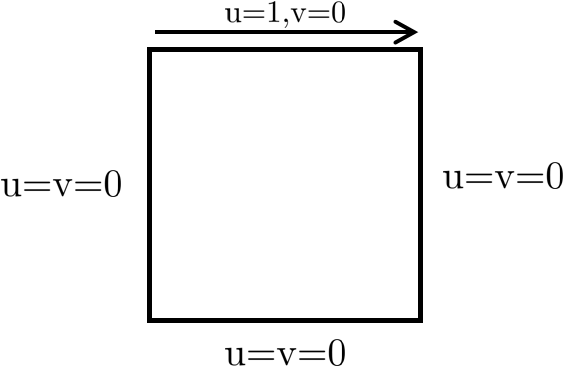
\includegraphics[width=0.35\textwidth]{Diagram}\caption{Diagram of model geometry \label{fig:Diagram}}
\end{figure}
In Figure \ref{fig:Diagram}, a basic diagram of the geometry is shown.
In this problem, the south, east, and west walls of the enclosure
are assumed to be stationary while the north wall is assumed to be
sliding in the positive x-direction with a non-dimensional velocity
of one.

\subsection{Governing Equations\label{subsec:Governing-Equations}}

In this work, it is assumed that the fluid within the cavity is not
rarefied and can be accurately considered to have both a constant
density and viscosity. With these assumptions, the two-dimensional
versions of the conservation of mass and conservation of momentum
can be simplified to the forms shown in Equations \ref{eq:ConMass},
\ref{eq:ConMomX}, and \ref{eq:ConMomY}. \nomenclature[u]{$u$}{velocity in x-direction}\nomenclature[v]{$v$}{velocity in y-direction}

\begin{equation}
\ensuremath{\frac{\partial u}{\partial x}+\frac{\partial v}{\partial y}=0}\label{eq:ConMass}
\end{equation}

\begin{equation}
\frac{\partial u}{\partial t}+\frac{\partial u^{2}}{\partial x}+\frac{\partial}{\partial y}\left(uv\right)+\frac{\partial P}{\partial x}=\frac{1}{\textmd{Re}}\left[\frac{\partial u^{2}}{\partial x^{2}}+\frac{\partial v^{2}}{\partial y}\right]\label{eq:ConMomX}
\end{equation}

\begin{equation}
\frac{\partial v}{\partial t}+\frac{\partial}{\partial x}\left(uv\right)+\frac{\partial v^{2}}{\partial y}+\frac{\partial P}{\partial y}=\frac{1}{\textmd{Re}}\left[\frac{\partial u^{2}}{\partial x^{2}}+\frac{\partial v^{2}}{\partial y}\right]\label{eq:ConMomY}
\end{equation}


\section{Solution Method}

\subsection{Projection Method}

Although the steady-state solution of the fluid pressure and velocity
is desired, a transient method is used to 

\begin{subequations}\label{eq:DiscTime}

\begin{equation}
\frac{\partial u}{\partial t}=\frac{u^{n+1}-u^{\star}}{\Delta t}\label{eq:DiscTimeX}
\end{equation}

\begin{equation}
\frac{\partial v}{\partial t}=\frac{v^{n+1}-v^{\star}}{\Delta t}\label{eq:DiscTimeY}
\end{equation}

\end{subequations}

\begin{subequations}\label{eq:Stars}

\begin{equation}
\frac{u^{\star}-u^{n}}{\Delta t}=-\frac{\partial u^{2}}{\partial x}-\frac{\partial}{\partial y}\left(uv\right)+\frac{1}{\textmd{Re}}\left[\frac{\partial u^{2}}{\partial x^{2}}+\frac{\partial v^{2}}{\partial y}\right]\label{eq:ustar}
\end{equation}

\begin{equation}
\frac{v^{\star}-v^{n}}{\Delta t}=-\frac{\partial v^{2}}{\partial y}-\frac{\partial}{\partial x}\left(uv\right)+\frac{1}{\textmd{Re}}\left[\frac{\partial u^{2}}{\partial x^{2}}+\frac{\partial v^{2}}{\partial y}\right]\label{eq:vstar}
\end{equation}

\end{subequations}

\begin{equation}
\left[\frac{\partial^{2}P}{\partial x^{2}}+\frac{\partial^{2}P}{\partial y^{2}}\right]^{n+1}=\frac{1}{\Delta t}\left[\frac{\partial u^{\star}}{\partial x}+\frac{\partial v^{\star}}{\partial y}\right]\label{eq:PoissonPressure}
\end{equation}

The method used to solve Equation \ref{eq:PoissonPressure} is described
in Section \ref{subsec:Poisson-Solver}. Once the equation is solv

\begin{subequations}\label{eq:N+1}

\begin{equation}
u_{i+\frac{1}{2},j}^{n+1}=u_{i+\frac{1}{2},j}^{\star}+\frac{\Delta t}{\Delta x}\left(P_{i+1,j}^{n+1}-P_{i.j}^{n+1}\right)\label{eq:uN+1}
\end{equation}

\begin{equation}
v_{i,j+\frac{1}{2}}^{n+1}=v_{i,j+\frac{1}{2}}^{\star}+\frac{\Delta t}{\Delta y}\left(P_{i,j+1}^{n+1}-P_{i.j}^{n+1}\right)\label{eq:vN+1}
\end{equation}

\end{subequations}

\subsection{Discretization and Boundary Conditions}

The governing equations of Section \ref{subsec:Governing-Equations}
were discretized using a staggered grid. Figure \ref{fig:Grid}shows
the node staggering method used in this work for an example grid consisting
of 25 interior pressure nodes. In theory, use of the staggered mesh
should eliminate any checkerboard error from occurring. In practice,
it was found that the additional complexity of incorporating the staggered
mesh into the computational algorithm actually often led to checkerboard
style error being observed in the results.

\begin{figure}
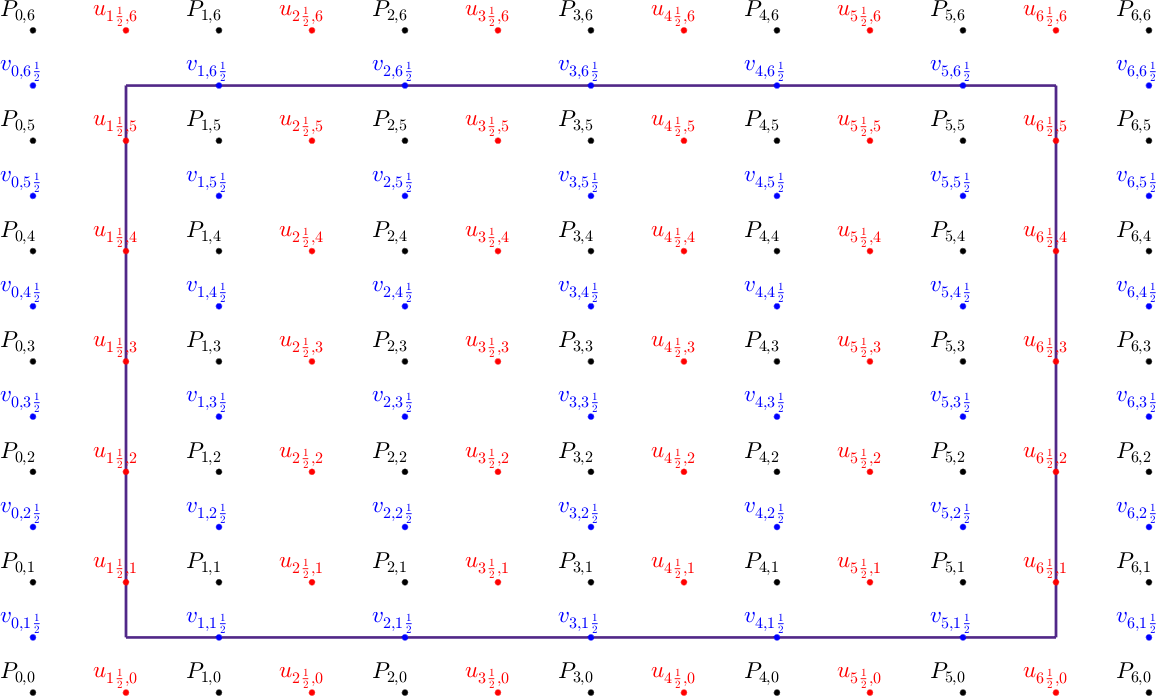
\includegraphics[width=0.5\textwidth]{SixPointGrid}\caption{Example of staggered grid \label{fig:Grid}}
\end{figure}
A central differencing scheme was used to discretize the derivatives
in Equations \ref{eq:DiscTime}\ref{eq:N+1}. Interpolation was used
whenever the scheme required information at a location between nodes.

Examples of this discretization for some of the terms in Equations
\ref{eq:DiscTime}\ref{eq:N+1} are given in Equations \ref{eq:DiscEx1}
and \ref{eq:DiscEx2}.

\begin{equation}
\left[\frac{\partial}{\partial x}\left(u^{2}\right)\right]_{i+\frac{1}{2},j}=\frac{\left(u_{i+1,j}\right)^{2}-\left(u_{i,j}\right)^{2}}{\Delta x}\label{eq:DiscEx1}
\end{equation}

\begin{equation}
\left[\frac{\partial}{\partial y}\left(uv\right)\right]_{i+\frac{1}{2},j}=\frac{\left(uv\right)_{i+\frac{1}{2},j+\frac{1}{2}}-\left(uv\right)_{i+\frac{1}{2},j-\frac{1}{2}}}{\Delta y}\label{eq:DiscEx2}
\end{equation}

For the $u$ and $v$ nodes, the nodes lying along their south, east,
and west boundaries were defined so that fluid velocity was zero at
the walls. If the outer velocity node was located outside of the cavity,
its value was defined so as the average between the outer node and
its nearest interior node was equal to zero. 

For the north boundary, a similar method was employed, however in
this case the outer $u$ velocity nodes were set so that the average
between themselves and their nearest interior node would be equal
to 1. The $v$ velocity nodes along the north boundary were again
set to zero, representing a no slip condition along the sliding wall.

\subsection{Poisson Solver\label{subsec:Poisson-Solver}}

Using the calculated $u^{\star}$and $v^{\star}$, the pressure Poisson
equation was solved using the Successive Over-Relaxation method.

\begin{equation}
C_{i,j}^{k}=\frac{1}{\Delta t}\left[\frac{u_{i+\frac{1}{2},j}^{\star}-u_{i-\frac{1}{2},j}^{\star}}{\Delta x}+\frac{v_{i,j+\frac{1}{2}}^{\star}-v_{i,j-\frac{1}{2}}^{\star}}{\Delta y}\right]\label{eq:C}
\end{equation}

\begin{multline}
\frac{P_{i+1,j}-2P_{i,j}+P_{i-1,j}}{\left(\Delta x\right)^{2}}+\frac{P_{i,j+1}-2P_{i,j}+P_{i,j-1}}{\left(\Delta y\right)^{2}}=C_{i,j}\label{eq:PressurePoisson}
\end{multline}

\[
\beta=\frac{\Delta x}{\Delta y}
\]

\begin{equation}
P_{i,j}^{k+1}=\left(1-\omega\right)P_{i,j}^{k}+\omega\frac{P_{i+1,j}^{k}+P_{i-1,j}^{k+1}+\beta^{2}\left(P_{i,j+1}^{k}+P_{i,j-1}^{k+1}\right)-\left(\Delta x\right)^{2}C_{i,j}^{k}}{2\left(1+\beta^{2}\right)}\label{eq:SOR}
\end{equation}

Equation \ref{eq:SOR} shows the general formula for the Successive
Over-Relaxation (SOR) method. The SOR method improves on the GS solution
method by incorporating over - or, if increased stability is desired,
under - relaxation into the equation using the relaxation parameter
$\omega$. When $\omega$ is equal to 1, the SOR method becomes identical
to the GS method. Raising $\omega$ to values greater than one can
increase the rate of convergence at the cost of stability. Conversely,
lowering the relaxation parameter below unity will result in dramatically
increased computational times, but provides greater stability. In
this work, values of $\omega$ of between .9 and 1.3 were used.

\section{Results - Part 1}

The inital conditons used and results obtained for part one can be
seen in Figure \ref{fig:Part1Solution}. In each of these figures,
the mesh used is overlayed.

\begin{figure}[h]
\centering%
\begin{minipage}[c]{0.49\textwidth}%
\subfloat[Part 1 initial conditions with mesh overlay\label{fig:Part1IC}]{\centering\includegraphics[clip,width=1\linewidth]{../../../Desktop/Project1/IC1}

}%
\end{minipage}\hfill{}\centering%
\begin{minipage}[c]{0.49\textwidth}%
\subfloat[Part one solution with mesh overlay \label{fig:Part1Psedo}]{\bigskip{}
\centering\includegraphics[clip,width=1\linewidth]{../../../Desktop/Project1/Solution1}

}%
\end{minipage}\caption{Solution of part 1 \label{fig:Part1Solution}}
\end{figure}

In Figure \ref{fig:ErrorPlots}, the effects each solver on the convergence
of the solution is shown. A convergence criteria of 1E-8 was used
solvers in this project.

\begin{figure}[h]
\centering%
\begin{minipage}[c]{0.49\textwidth}%
\subfloat[Error vs iteration number for each solver\label{fig:Norm2Error}]{\centering\includegraphics[clip,width=1\linewidth]{../../../Desktop/Project1/ErrorCompare1}

}%
\end{minipage}\hfill{}\centering%
\begin{minipage}[c]{0.49\textwidth}%
\subfloat[Comparison of norm 1, norm 2, norm$\infty$ error\label{fig:ErrorCompare}]{\centering\includegraphics[clip,width=1\linewidth]{../../../Desktop/Project1/NormCompare1}

}%
\end{minipage}\caption{Relative error from examined solution methods \label{fig:ErrorPlots}}
\end{figure}

\begin{table}
\centering

\begin{tabular}{|c|c|c|c|c|c|}
\hline 
 & \textbf{Jacobi} & \textbf{G-S} & \textbf{SOR} & \textbf{SLOR} & \textbf{ADI}\tabularnewline
\hline 
\textbf{Time per Iteration {[}s{]}} & 5.75E-5 & 5.78E-5 & 6.58E-5 & 2.0E-4 & 2.34E-4\tabularnewline
\hline 
\textbf{Solution Time {[}s{]}} & 6.5E-2 & 3.4E-2 & 4.5E-3 & 1.0E-2 & 7.25E-3\tabularnewline
\hline 
\textbf{Optimal $\omega$} & N/A & N/A & 1.7189 & 1.2421 & 1.3\tabularnewline
\hline 
\textbf{Minimum Iterations} & 1127 & 592 & 68 & 50 & 31\tabularnewline
\hline 
\end{tabular}\caption{Solver effectiveness \label{tab:SolverTable}}

\end{table}

\begin{table}

\begin{tabular}{|c|c|c|c|c|c|c|}
\hline 
 &  & dt & dx & Nodes & Tolerance & Computational Time\tabularnewline
\hline 
 & 1 &  &  &  &  & \tabularnewline
\cline{2-7} 
 & 10 &  &  &  &  & \tabularnewline
\cline{2-7} 
 & 100 &  &  &  &  & \tabularnewline
\cline{2-7} 
Re & 400 &  &  &  &  & \tabularnewline
\cline{2-7} 
 & 400 & 2.0E-4 &  &  &  & \tabularnewline
\cline{2-7} 
 & 400 & 0.005 & 0.0101 & 100x100 & 5.0E-7 & 270\tabularnewline
\cline{2-7} 
 & 1000 & 0.0036 & 0.0204 & 50x50 & 5.0E-7 & 363\tabularnewline
\hline 
\end{tabular}\caption{Results}

\end{table}

For the second part of the this project, the box geometry was modified
so that a portion of the right corner was removed. The line defining
the removed corner is shown as the dotted line in \ref{fig:Diagram}.
This change in the size of the domain was implemented by adjusting
the initial conditions and boundary conditions used when solving for
$\psi$. The new wall was applied by initially assigning all nodes
beyond the new boundary line as boundary nodes possessing constant
values of $\omega=1$. A visual depiction of this application can
be seen in Figure \ref{fig:Re1u}.

The restricted domain was seen to slightly modify the stream function
calculated within the domain. This change can be seen in Figure \ref{fig:Re1v}
in which the a contour plot with the results from the geometry of
part 1 is overlayed with the new results from the domain with the
removed corner. In Figure \ref{fig:Re1v}, the black contours are
those from the geometry of part 1, and the colored contours are from
the results calculated with the new geometry.

\begin{figure}[h]
\centering%
\begin{minipage}[c]{0.49\textwidth}%
\subfloat[$u$\label{fig:Re1u}]{\centering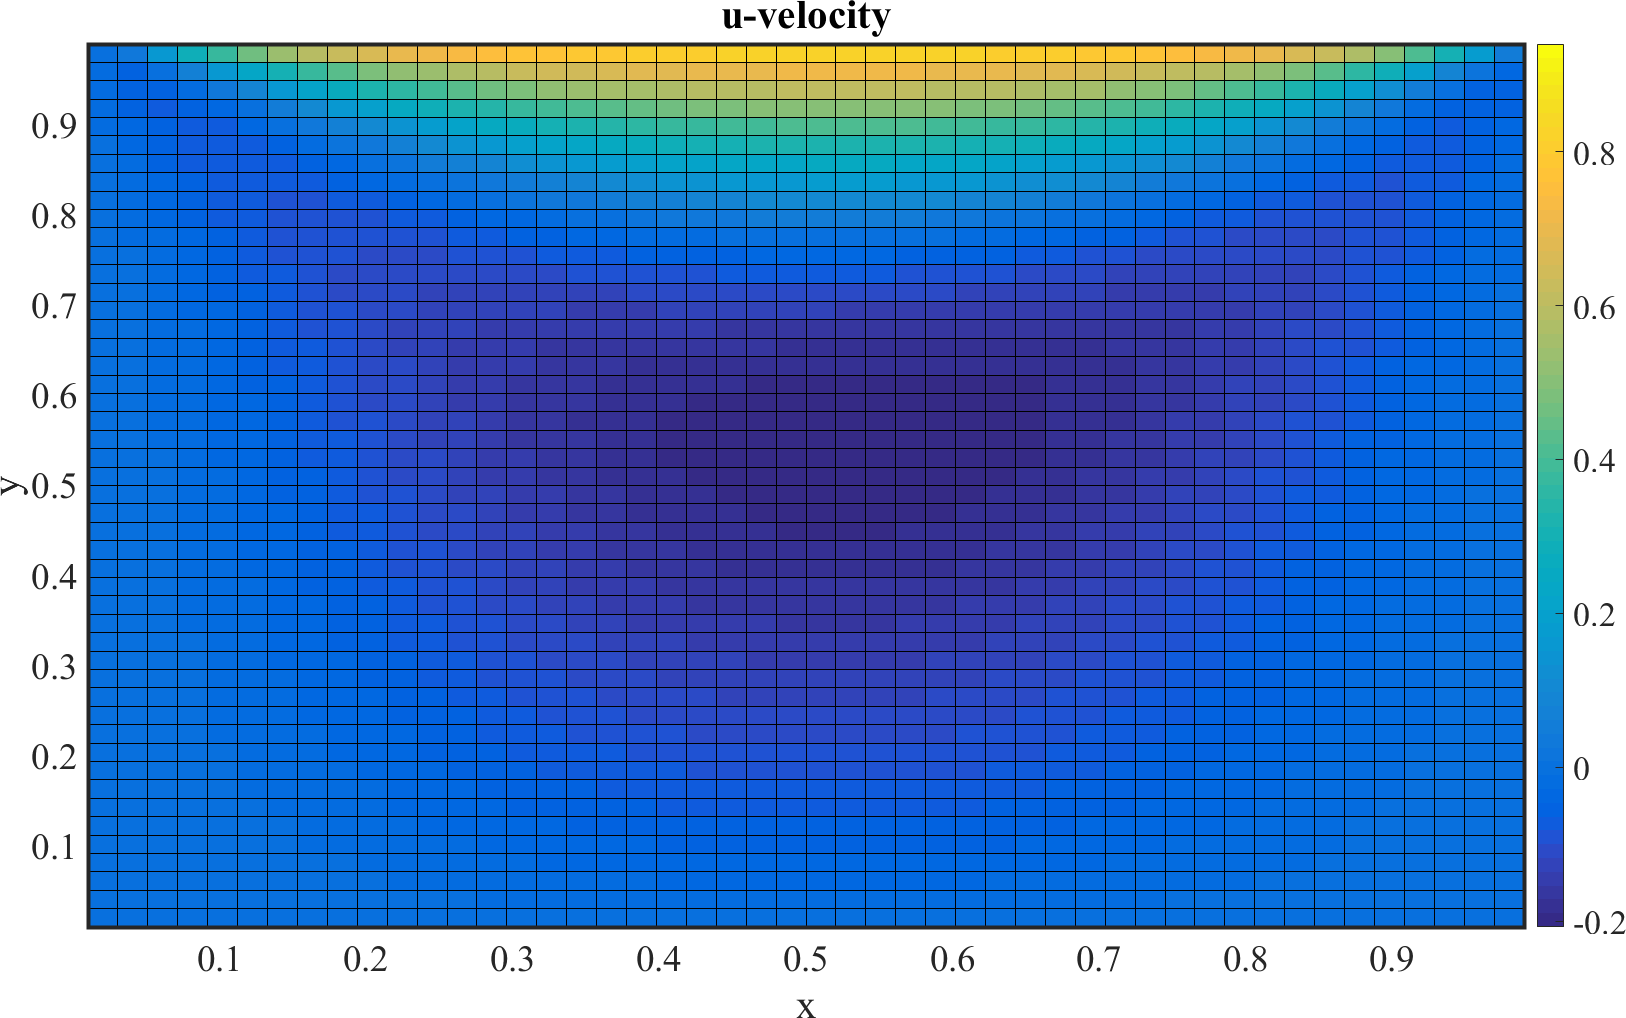
\includegraphics[clip,width=1\linewidth]{Re10u}

}%
\end{minipage}\hfill{}\centering%
\begin{minipage}[c]{0.49\textwidth}%
\subfloat[$v$\label{fig:Re1v}]{\centering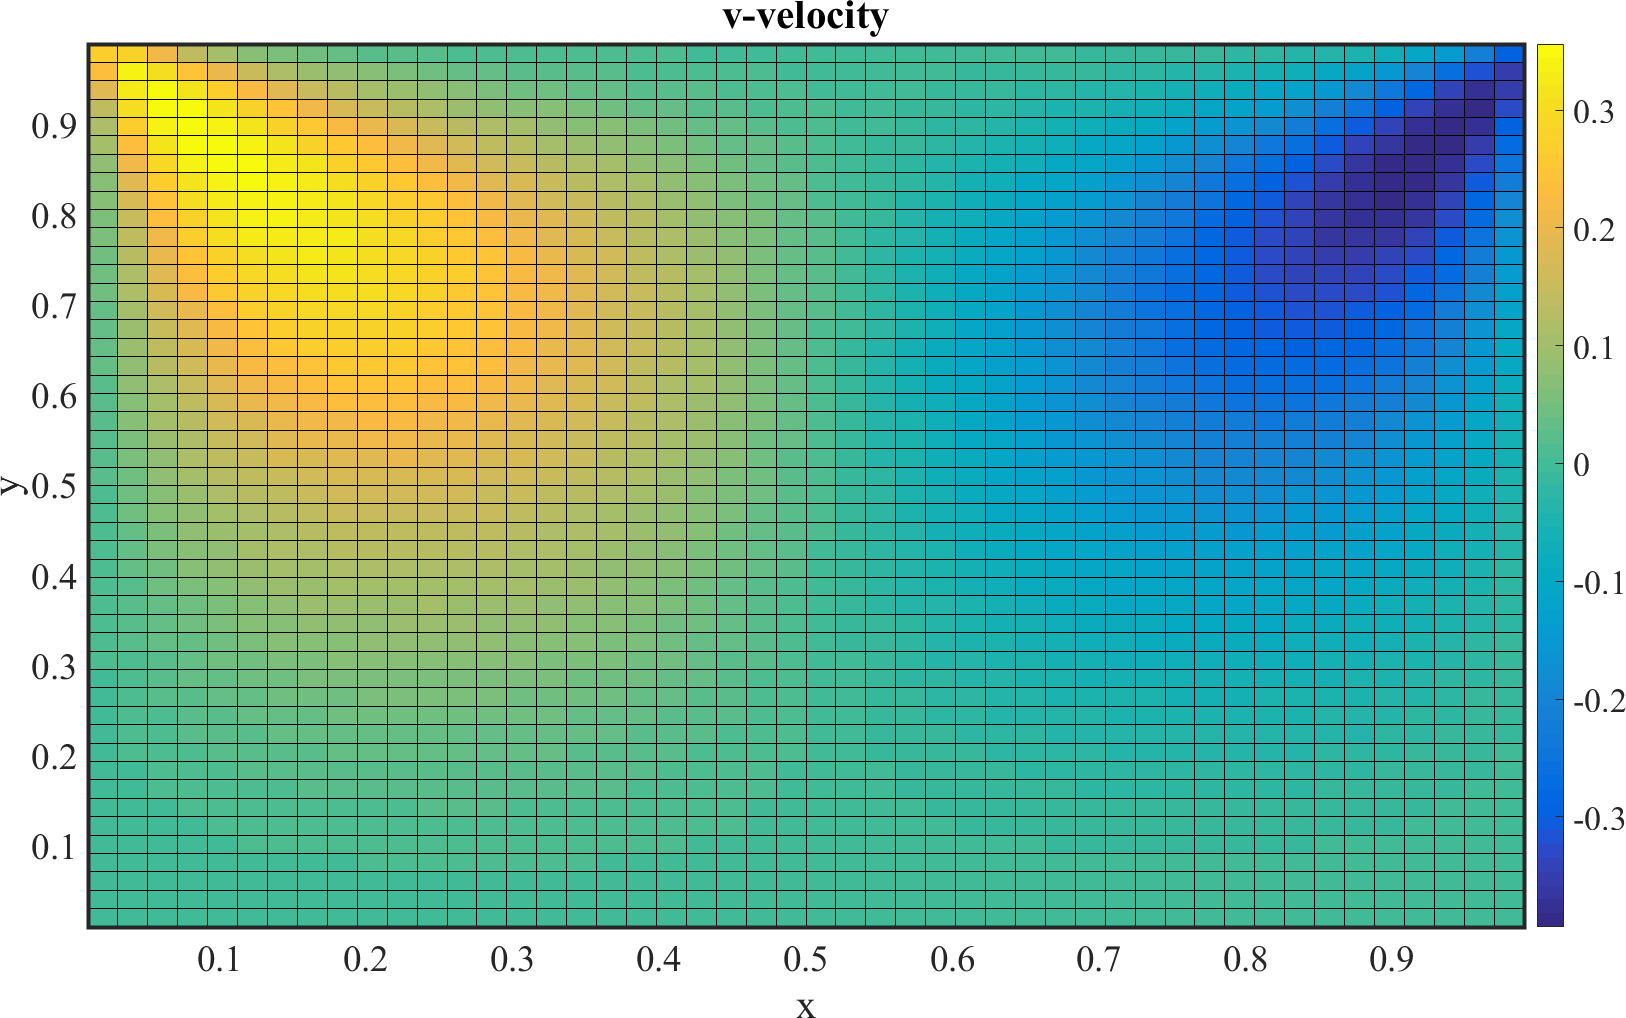
\includegraphics[clip,width=1\linewidth]{Re10v}

}%
\end{minipage}\medskip{}

\centering%
\begin{minipage}[c]{0.49\textwidth}%
\subfloat[Flow Speed \label{fig:Re1Speed}]{\centering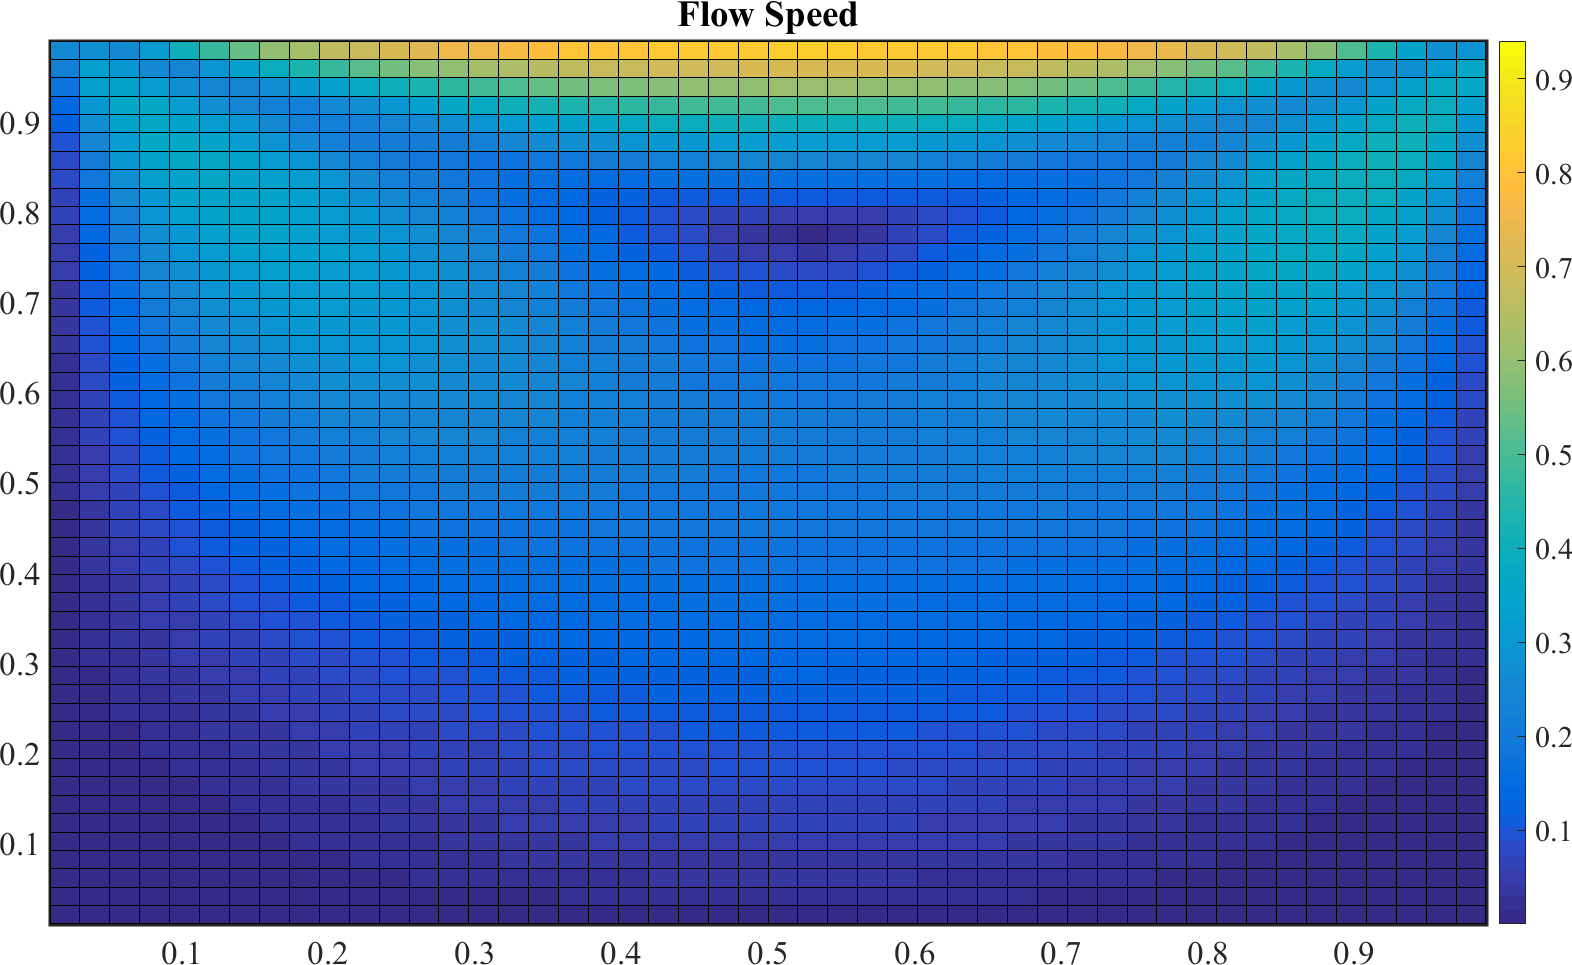
\includegraphics[clip,width=1\linewidth]{Re10Speed}

}%
\end{minipage}\hfill{}\centering%
\begin{minipage}[c]{0.49\textwidth}%
\subfloat[$\psi$\label{fig:Re1Stream}]{\centering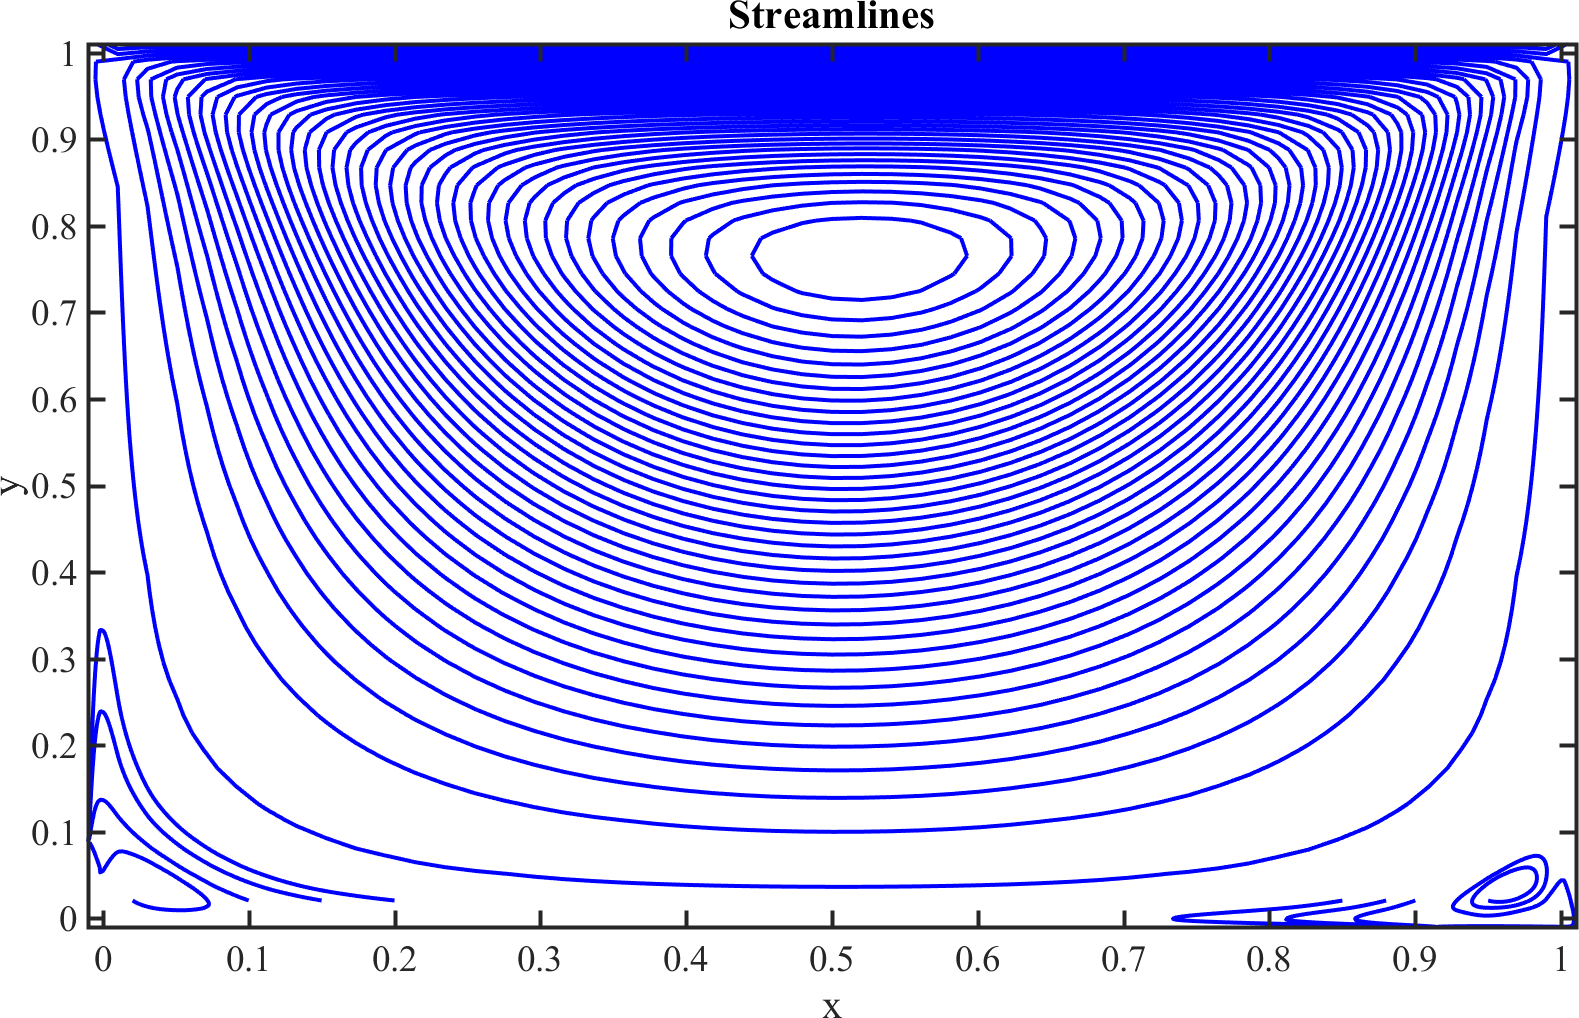
\includegraphics[clip,width=1\linewidth]{Re10Stream}

}%
\end{minipage}\caption{Results - Re 10\label{fig:Re1Results}}
\end{figure}

\begin{figure}[h]
\centering%
\begin{minipage}[c]{0.49\textwidth}%
\subfloat[$u$\label{fig:Re1u-1}]{\centering\includegraphics[clip,width=1\linewidth]{../../../Desktop/Project1/IC2}

}%
\end{minipage}\hfill{}\centering%
\begin{minipage}[c]{0.49\textwidth}%
\subfloat[$v$\label{fig:Re1v-1}]{\centering\includegraphics[clip,width=1\linewidth]{../../../Desktop/Project1/ContourCompare}

}%
\end{minipage}\medskip{}

\centering%
\begin{minipage}[c]{0.49\textwidth}%
\subfloat[Flow Speed \label{fig:Re1Speed-1}]{\centering\includegraphics[clip,width=1\linewidth]{../../../Desktop/Project1/IC2}

}%
\end{minipage}\hfill{}\centering%
\begin{minipage}[c]{0.49\textwidth}%
\subfloat[$\psi$\label{fig:Re1Stream-1}]{\centering\includegraphics[clip,width=1\linewidth]{../../../Desktop/Project1/ContourCompare}

}%
\end{minipage}\caption{Results - Re 100\label{fig:Re10Results}}
\end{figure}

\begin{figure}[h]
\centering%
\begin{minipage}[c]{0.49\textwidth}%
\subfloat[$u$\label{fig:Re1u-2}]{\centering\includegraphics[clip,width=1\linewidth]{../../../Desktop/Project1/IC2}

}%
\end{minipage}\hfill{}\centering%
\begin{minipage}[c]{0.49\textwidth}%
\subfloat[$v$\label{fig:Re1v-2}]{\centering\includegraphics[clip,width=1\linewidth]{../../../Desktop/Project1/ContourCompare}

}%
\end{minipage}\medskip{}

\centering%
\begin{minipage}[c]{0.49\textwidth}%
\subfloat[Flow Speed \label{fig:Re1Speed-2}]{\centering\includegraphics[clip,width=1\linewidth]{../../../Desktop/Project1/IC2}

}%
\end{minipage}\hfill{}\centering%
\begin{minipage}[c]{0.49\textwidth}%
\subfloat[$\psi$\label{fig:Re400Stream}]{\centering\includegraphics[clip,width=1\linewidth]{../../../Desktop/Project1/ContourCompare}

}%
\end{minipage}\caption{Results - Re 400\label{fig:Re400Results}}
\end{figure}

\begin{figure}[h]
\centering%
\begin{minipage}[c]{0.49\textwidth}%
\subfloat[$u$\label{fig:Re1u-3}]{\centering\includegraphics[clip,width=1\linewidth]{../../../Desktop/Project1/IC2}

}%
\end{minipage}\hfill{}\centering%
\begin{minipage}[c]{0.49\textwidth}%
\subfloat[$v$\label{fig:Re1v-3}]{\centering\includegraphics[clip,width=1\linewidth]{../../../Desktop/Project1/ContourCompare}

}%
\end{minipage}\medskip{}

\centering%
\begin{minipage}[c]{0.49\textwidth}%
\subfloat[Flow Speed \label{fig:Re1000Speed}]{\centering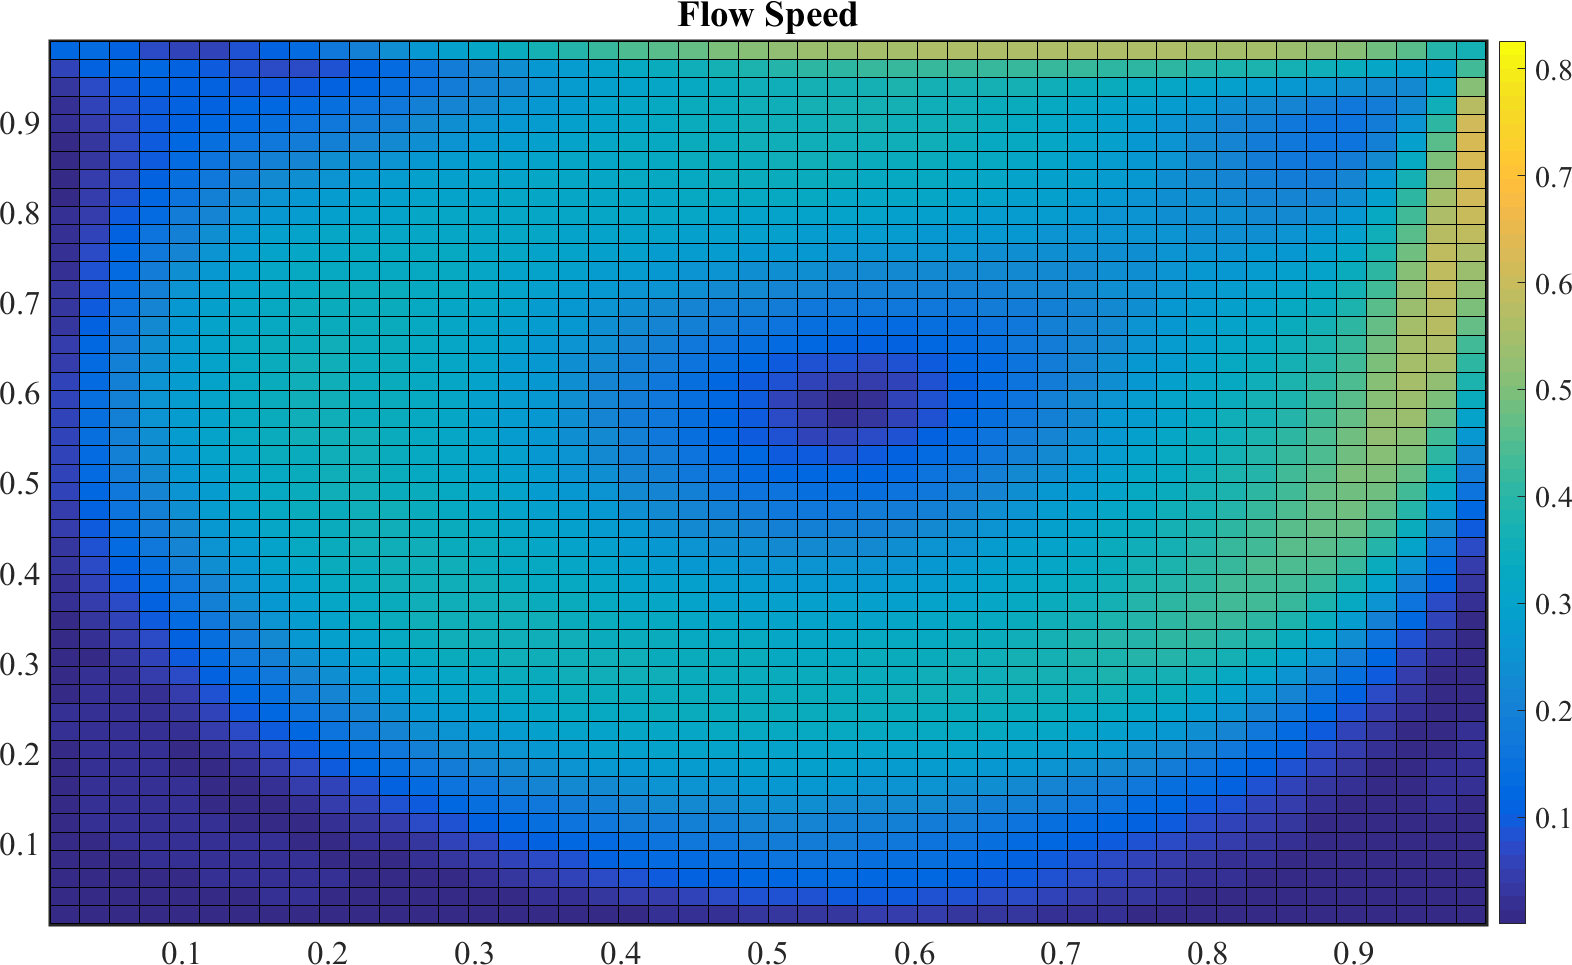
\includegraphics[clip,width=1\linewidth]{Re1000Speed}

}%
\end{minipage}\hfill{}\centering%
\begin{minipage}[c]{0.49\textwidth}%
\subfloat[$\psi$\label{fig:Re1000Stream}]{\centering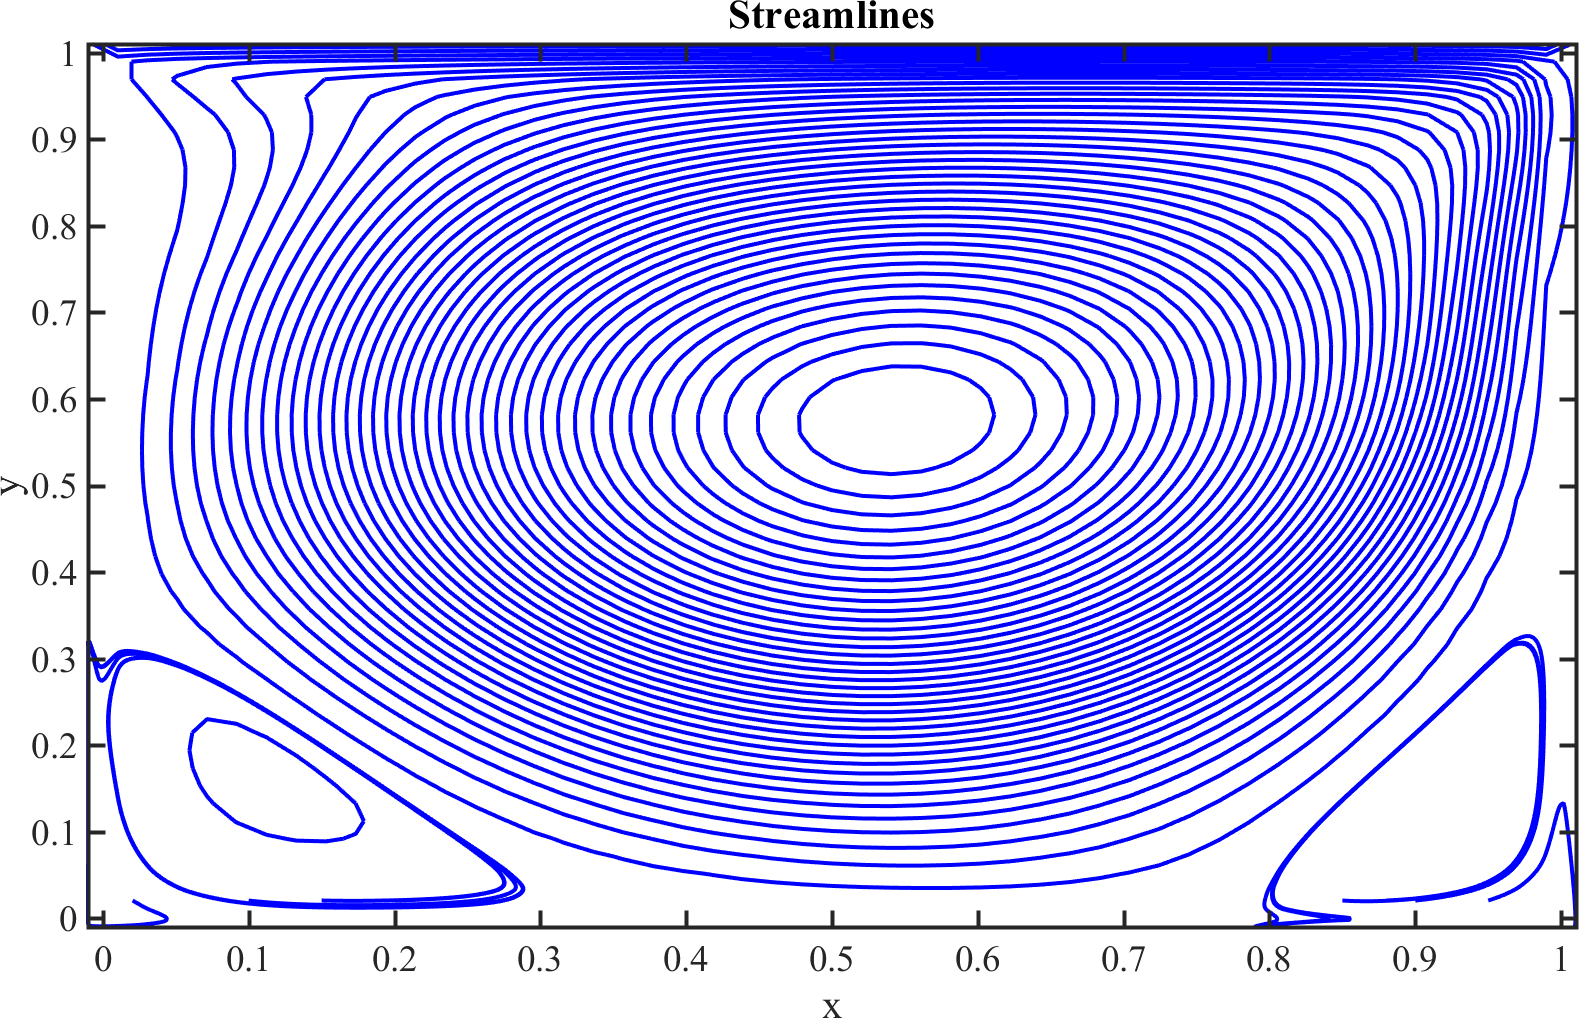
\includegraphics[clip,width=1\linewidth]{Re1000Stream}

}%
\end{minipage}\caption{Results - Re 1000\label{fig:Re1000Results}}
\end{figure}

While Figure \ref{fig:Re1v} does make it clear that \textit{some
}change in the results did indeed occur due to the modified corner
boundary, in order to both better understand the effect of geometry
on the flow patterns within the box and provided validation for the
geometry adjustment method used, the domain of analysis was further
restricted by removing all nodes beyond the boundary identified in
Figure \ref{fig:Diagram} as the ``Modified Wall''. Unsurprisingly,
moving the wall this far into the domain proved to have a much larger
effect.

\begin{figure}[h]
\centering%
\begin{minipage}[c]{0.49\textwidth}%
\subfloat[Re 400\label{fig:CenterlineCompare400}]{\centering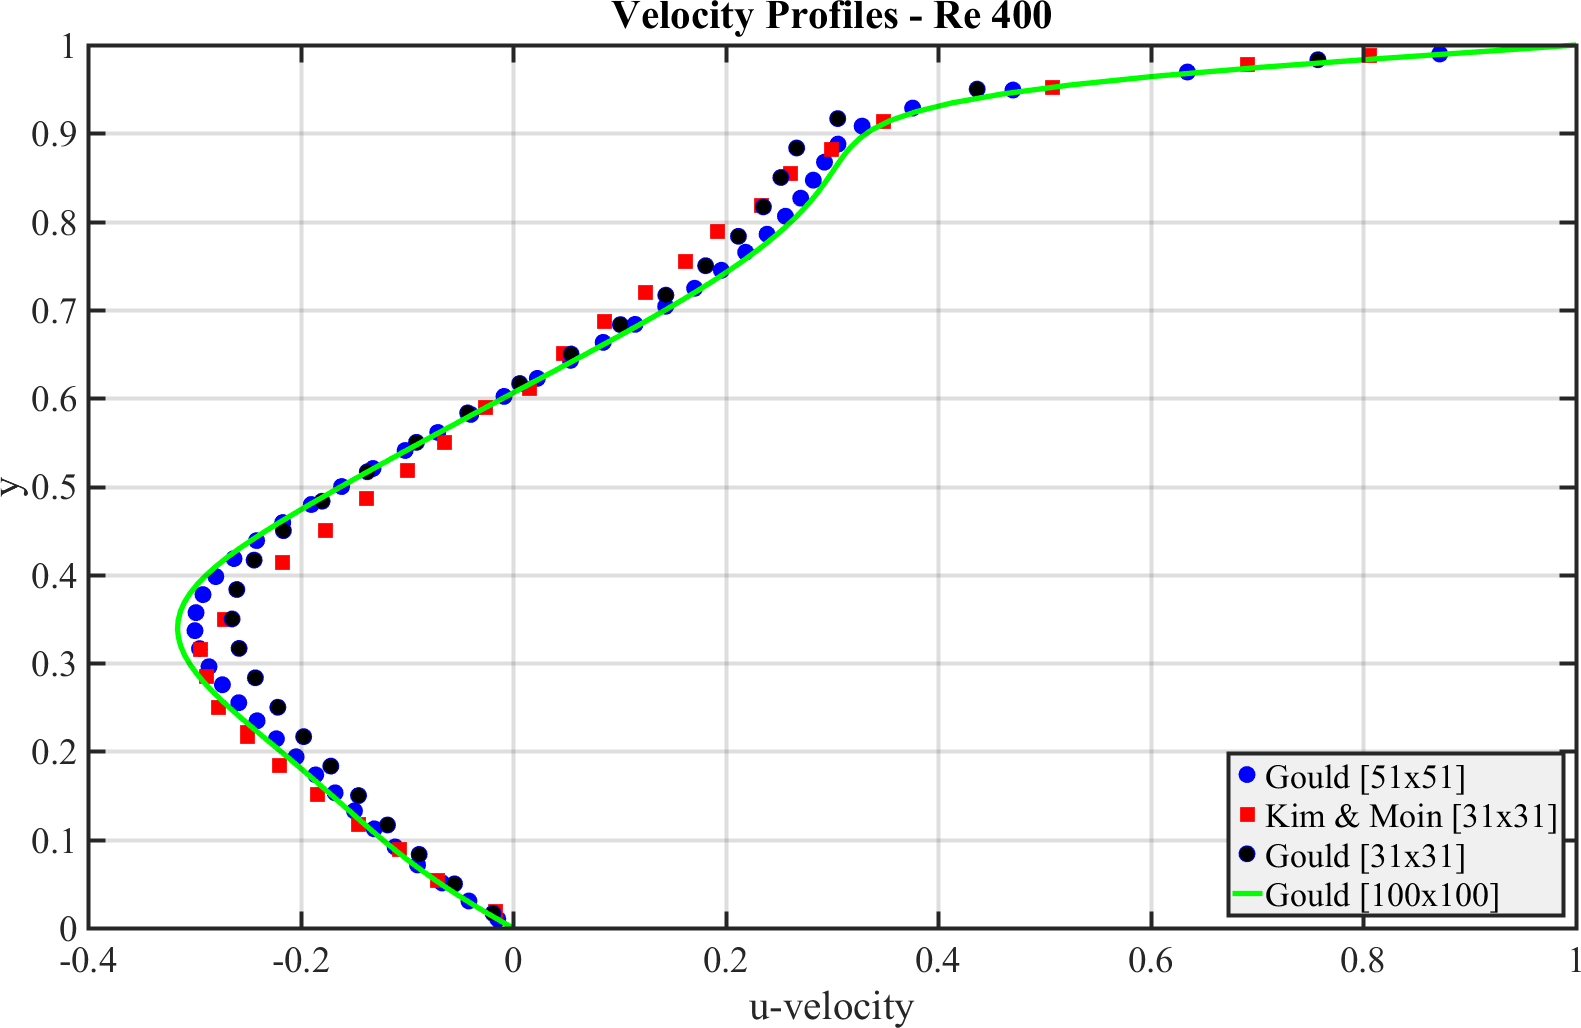
\includegraphics[clip,width=1\linewidth]{Re400profiles}

}%
\end{minipage}\hfill{}\centering%
\begin{minipage}[c]{0.49\textwidth}%
\subfloat[Re400\label{fig:CenterlineCompare1000}]{\centering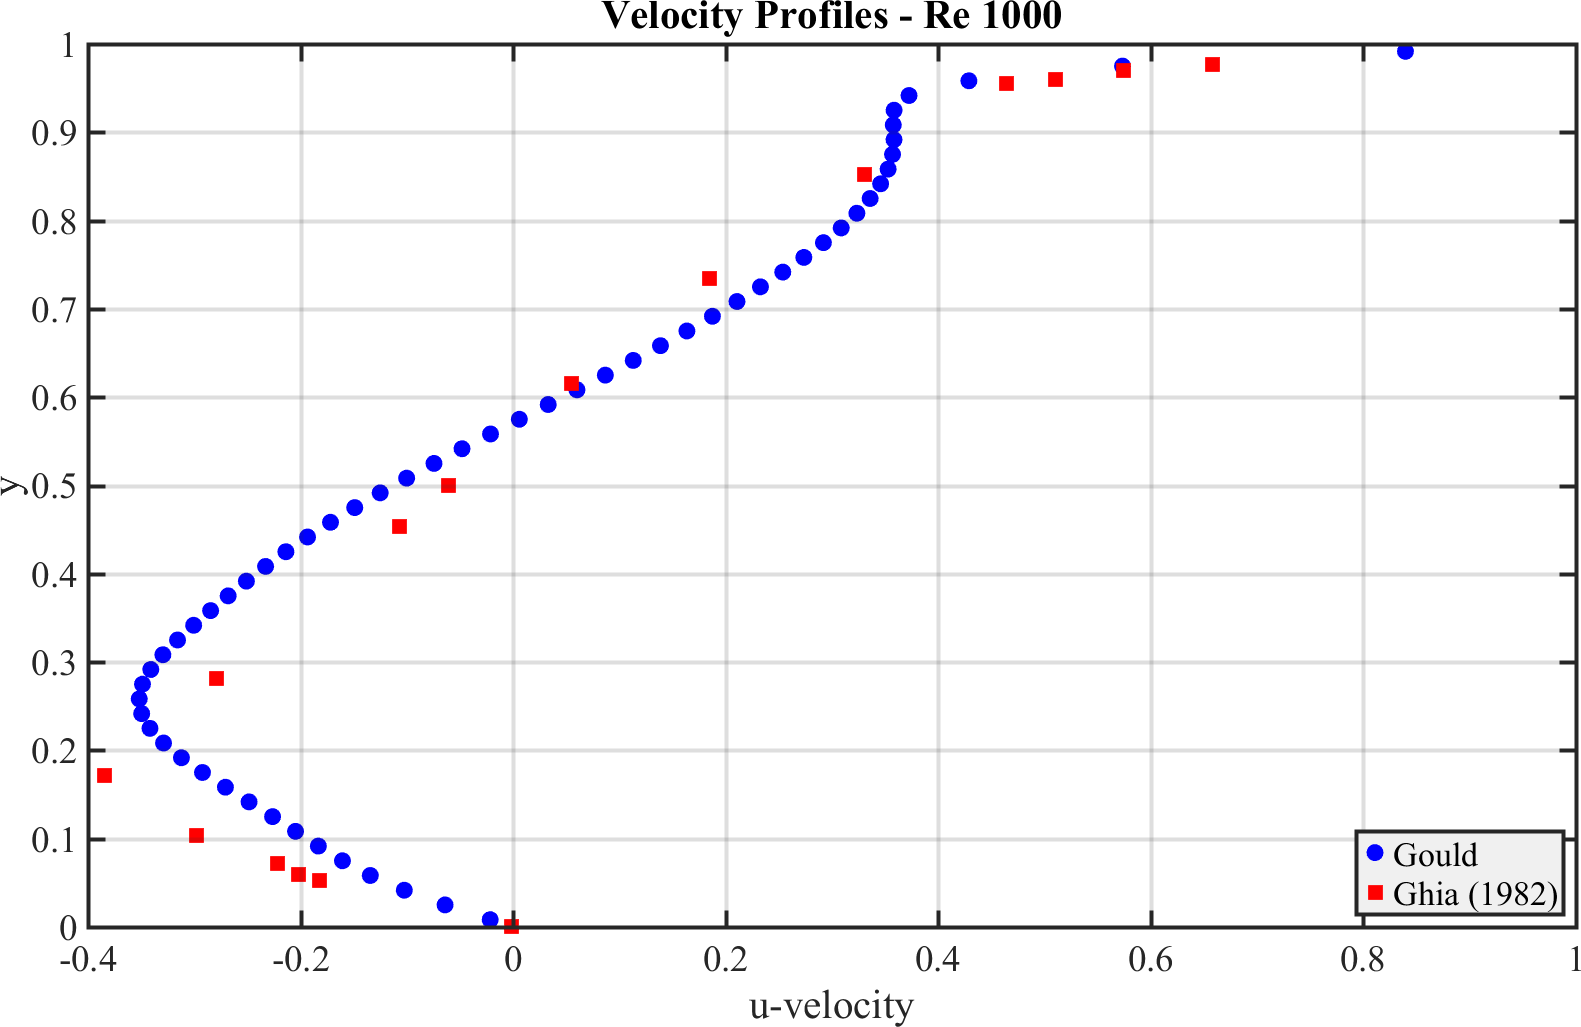
\includegraphics[clip,width=1\linewidth]{CenterlineVelocityRe1000}

}%
\end{minipage}\caption{Comparison of calculated $u$ velocity along cavity centerline \label{fig:CenterlineCompare}}
\end{figure}

Finally, to further disturb the flow, a partial barrier was added
in the region between the inlet and outlet by assigning a line of
nodes at x=3m to be equal 0. This assignment created a new wall attached
to the wall between points A and C. This is seen in Figure \ref{fig:ICbarrier}.
Unsurprisingly, the addition of the barrier worked in conjunction
with the extended wall and resulted in a highly disturbed flow path.
A contour and pseudocolor plot depicting this is presented in Figure
\ref{fig:imageContour}. The code calculating this effect is provided
in Appendix \ref{subsec:Problem-2-w/}.

\begin{figure}[h]
\centering%
\begin{minipage}[c]{0.49\textwidth}%
\subfloat[Initial conditions for simulation with barrier\label{fig:ICbarrier}]{\centering\includegraphics[clip,width=1\linewidth]{../../../Desktop/Project1/ICBarrier}

}%
\end{minipage}\hfill{}\centering%
\begin{minipage}[c]{0.49\textwidth}%
\subfloat[Effect of barrier on solution \label{fig:imageContour}]{\centering\includegraphics[clip,width=1\linewidth]{../../../Desktop/Project1/SolutionBarrierContour}

}%
\end{minipage}\caption{Modified geometry - shape and barrier \label{fig:Barrier}}
\end{figure}


\section{Conclusion}

Despite the limited resolution, the methods employed in solving the
Laplace equation for the stream function within the domain of interest
proved to be very effective. Regarding the different solution methods,
it was found that when using Matlab, the ability to vectorize an equation
is of significant importance. This is admittedly a significant drawback
if one is going to be using the language for iterative solutions to
finite difference equations. Unfortunately, it was also discovered
by the author that all other coding options are horrible and evil.
Thus, in the future, this author would recommend that FDE equations
can be best solved by either using working in Matlab and using Matlab's
built in, vectorized functions as much as possible, or simply buying
some computer science grad student a 6 pack of beer to program the
solution code for you in a awful, but fast language such as C or Fortran.
\end{document}
